% Options for packages loaded elsewhere
\PassOptionsToPackage{unicode}{hyperref}
\PassOptionsToPackage{hyphens}{url}
%
\documentclass[
  english,
  ,jou,floatsintext]{apa6}
\usepackage{amsmath,amssymb}
\usepackage{lmodern}
\usepackage{iftex}
\ifPDFTeX
  \usepackage[T1]{fontenc}
  \usepackage[utf8]{inputenc}
  \usepackage{textcomp} % provide euro and other symbols
\else % if luatex or xetex
  \usepackage{unicode-math}
  \defaultfontfeatures{Scale=MatchLowercase}
  \defaultfontfeatures[\rmfamily]{Ligatures=TeX,Scale=1}
\fi
% Use upquote if available, for straight quotes in verbatim environments
\IfFileExists{upquote.sty}{\usepackage{upquote}}{}
\IfFileExists{microtype.sty}{% use microtype if available
  \usepackage[]{microtype}
  \UseMicrotypeSet[protrusion]{basicmath} % disable protrusion for tt fonts
}{}
\makeatletter
\@ifundefined{KOMAClassName}{% if non-KOMA class
  \IfFileExists{parskip.sty}{%
    \usepackage{parskip}
  }{% else
    \setlength{\parindent}{0pt}
    \setlength{\parskip}{6pt plus 2pt minus 1pt}}
}{% if KOMA class
  \KOMAoptions{parskip=half}}
\makeatother
\usepackage{xcolor}
\IfFileExists{xurl.sty}{\usepackage{xurl}}{} % add URL line breaks if available
\IfFileExists{bookmark.sty}{\usepackage{bookmark}}{\usepackage{hyperref}}
\hypersetup{
  pdftitle={Changing coronavirus vaccination attitudes},
  pdfauthor={Charlotte Brand1 \& Tom Stafford2},
  pdflang={en-EN},
  hidelinks,
  pdfcreator={LaTeX via pandoc}}
\urlstyle{same} % disable monospaced font for URLs
\usepackage{graphicx}
\makeatletter
\def\maxwidth{\ifdim\Gin@nat@width>\linewidth\linewidth\else\Gin@nat@width\fi}
\def\maxheight{\ifdim\Gin@nat@height>\textheight\textheight\else\Gin@nat@height\fi}
\makeatother
% Scale images if necessary, so that they will not overflow the page
% margins by default, and it is still possible to overwrite the defaults
% using explicit options in \includegraphics[width, height, ...]{}
\setkeys{Gin}{width=\maxwidth,height=\maxheight,keepaspectratio}
% Set default figure placement to htbp
\makeatletter
\def\fps@figure{htbp}
\makeatother
\setlength{\emergencystretch}{3em} % prevent overfull lines
\providecommand{\tightlist}{%
  \setlength{\itemsep}{0pt}\setlength{\parskip}{0pt}}
\setcounter{secnumdepth}{-\maxdimen} % remove section numbering
% Make \paragraph and \subparagraph free-standing
\ifx\paragraph\undefined\else
  \let\oldparagraph\paragraph
  \renewcommand{\paragraph}[1]{\oldparagraph{#1}\mbox{}}
\fi
\ifx\subparagraph\undefined\else
  \let\oldsubparagraph\subparagraph
  \renewcommand{\subparagraph}[1]{\oldsubparagraph{#1}\mbox{}}
\fi
\newlength{\cslhangindent}
\setlength{\cslhangindent}{1.5em}
\newlength{\csllabelwidth}
\setlength{\csllabelwidth}{3em}
\newlength{\cslentryspacingunit} % times entry-spacing
\setlength{\cslentryspacingunit}{\parskip}
\newenvironment{CSLReferences}[2] % #1 hanging-ident, #2 entry spacing
 {% don't indent paragraphs
  \setlength{\parindent}{0pt}
  % turn on hanging indent if param 1 is 1
  \ifodd #1
  \let\oldpar\par
  \def\par{\hangindent=\cslhangindent\oldpar}
  \fi
  % set entry spacing
  \setlength{\parskip}{#2\cslentryspacingunit}
 }%
 {}
\usepackage{calc}
\newcommand{\CSLBlock}[1]{#1\hfill\break}
\newcommand{\CSLLeftMargin}[1]{\parbox[t]{\csllabelwidth}{#1}}
\newcommand{\CSLRightInline}[1]{\parbox[t]{\linewidth - \csllabelwidth}{#1}\break}
\newcommand{\CSLIndent}[1]{\hspace{\cslhangindent}#1}
% Manuscript styling
\usepackage{upgreek}
\captionsetup{font=singlespacing,justification=justified}

% Table formatting
\usepackage{longtable}
\usepackage{lscape}
% \usepackage[counterclockwise]{rotating}   % Landscape page setup for large tables
\usepackage{multirow}		% Table styling
\usepackage{tabularx}		% Control Column width
\usepackage[flushleft]{threeparttable}	% Allows for three part tables with a specified notes section
\usepackage{threeparttablex}            % Lets threeparttable work with longtable

% Create new environments so endfloat can handle them
% \newenvironment{ltable}
%   {\begin{landscape}\centering\begin{threeparttable}}
%   {\end{threeparttable}\end{landscape}}
\newenvironment{lltable}{\begin{landscape}\centering\begin{ThreePartTable}}{\end{ThreePartTable}\end{landscape}}

% Enables adjusting longtable caption width to table width
% Solution found at http://golatex.de/longtable-mit-caption-so-breit-wie-die-tabelle-t15767.html
\makeatletter
\newcommand\LastLTentrywidth{1em}
\newlength\longtablewidth
\setlength{\longtablewidth}{1in}
\newcommand{\getlongtablewidth}{\begingroup \ifcsname LT@\roman{LT@tables}\endcsname \global\longtablewidth=0pt \renewcommand{\LT@entry}[2]{\global\advance\longtablewidth by ##2\relax\gdef\LastLTentrywidth{##2}}\@nameuse{LT@\roman{LT@tables}} \fi \endgroup}

% \setlength{\parindent}{0.5in}
% \setlength{\parskip}{0pt plus 0pt minus 0pt}

% \usepackage{etoolbox}
\makeatletter
\patchcmd{\HyOrg@maketitle}
  {\section{\normalfont\normalsize\abstractname}}
  {\section*{\normalfont\normalsize\abstractname}}
  {}{\typeout{Failed to patch abstract.}}
\patchcmd{\HyOrg@maketitle}
  {\section{\protect\normalfont{\@title}}}
  {\section*{\protect\normalfont{\@title}}}
  {}{\typeout{Failed to patch title.}}
\makeatother
\shorttitle{Clickbot replication}
\usepackage{dblfloatfix}


\usepackage{csquotes}
\ifXeTeX
  % Load polyglossia as late as possible: uses bidi with RTL langages (e.g. Hebrew, Arabic)
  \usepackage{polyglossia}
  \setmainlanguage[]{english}
\else
  \usepackage[main=english]{babel}
% get rid of language-specific shorthands (see #6817):
\let\LanguageShortHands\languageshorthands
\def\languageshorthands#1{}
\fi
\ifLuaTeX
  \usepackage{selnolig}  % disable illegal ligatures
\fi

\title{Changing coronavirus vaccination attitudes}
\author{Charlotte Brand\textsuperscript{1} \& Tom Stafford\textsuperscript{2}}
\date{}


\note{\textcolor{red}{This paper is a pre-print and has not yet been peer-reviewed}}

\authornote{

Contents of this author note autogenerated using Tenzing \url{https://martonbalazskovacs.shinyapps.io/tenzing/}

The authors made the following contributions. Charlotte Brand: Conceptualization, Project Administration, Data collection and analysis, Visualization, Writing - Original Draft Preparation, Writing - Review \& Editing; Tom Stafford: Conceptualization, Funding Acquisition, Writing - Review \& Editing.

Correspondence concerning this article should be addressed to Charlotte Brand, Enter postal address here. E-mail: \href{mailto:c.brand@sheffield.ac.uk}{\nolinkurl{c.brand@sheffield.ac.uk}}

}

\affiliation{\vspace{0.5cm}\textsuperscript{1} University of Sheffield\\\textsuperscript{2} University of Sheffield}

\abstract{
A recent study found that interacting with a chatbot for around five minutes led to an increase in Covid-19 vaccination attitudes and intentions in a French population, compared to a control condition (Altay et al.~2020). We wanted test this effect with a UK population whilst making some key modifications. Firstly we wanted to control the amount of information provided by the chatbot compared to the control condition, as well as the time spent with the information, how the trustworthiness of the information was communicated, and the interactivity of the information. By isolating the effect of the `choice of information' in our experimental condition, we wished to discover what it was about the chatbot that was more effective than their control. In our control condition, participants were randomly exposed to four dialogues of Covid-19 vaccination information in a Q\&A format of 200-500 words each, each containing two-three follow-up questions. Our experimental condition differed only in that participants could choose the four dialogues they were exposed to, and were given a choice of Five Question topics to choose from. Like the Altay Chatbot, we saw an increase in positive attitudes towards vaccination, as well as an increase in intention to get vaccinated, after viewing the information. Crucially, we found no difference in our conditions, in that choosing the questions did not increase vaccine attitudes, nor did it increase vaccine intentions, compared to randomly displaying the information. This is in contrast to Altay's experiment in which the Chatbot had a significantly greater effect than their Control. Importantly, in Altay's experiment their Control condition a) consisted of significantly less information b) did not provide information about the trustworthiness of the information and c) led to participants spending less time with the information. Similarly to the previous study, we also found an effect of time spent with the information, across both conditions, in that those who spent between 4 and 16 minutes (above the median) with the information were more likely to increase both their attitudes and their vaccination intentions. Another crucial difference is our sample, in that we specifically targeted those who were already either against or neutral towards covid-19 vaccinations specifically, and screened-out any who were already positive towards covid-19 vaccinations
}



\begin{document}
\maketitle

\begin{verbatim}
## Warning: package 'knitr' was built under R version 3.6.2
\end{verbatim}

\begin{verbatim}
## Warning: package 'ggplot2' was built under R version 3.6.2
\end{verbatim}

\hypertarget{introduction}{%
\section{Introduction}\label{introduction}}

You will find it useful to add 3 and 5 to make 8 compare the output PDF document with the .rmd document. This latter item is the thing you edit to produce the PDF.

Communicating the effectiveness, necessity and safety of vaccination to the general public is arguably one of science communication's most important and emblematic challenges. Appropriately, huge amounts of attention and research effort has been directed towards how to increase Covid-19 vaccination uptake. Due to the urgency and impact of the problem, a multi-pronged attack is warranted, and thus research rightly spans many different strategies, from pre-empting misinformation on social media (Vraga \& Bode 2021), presenting information on the comparison of Covid-19 symptoms to vaccination side-effects (Thorpe et al.~2021), presenting information on the timeline of vaccine development (Thorpe et al.~2021), different styles of myth-busting (Challenger et al.~20201), the use of social norms (Moehring et al.~2021) and even chatbots (Altay et al.~2020), all with varying levels of success.

Do I need a para here about chatbots in general? Usually used for tasks, only just starting to have real interest in their ability to have constructive dialogue etc? Check Altay's GMO chatbot paper intro for inspo.

Here we focus on the use of chatbots for attitude change. The use of chatbots to change attitudes is not restricted to vaccination hesitancy, and has previously been explored in the context of GMO attitudes (Altay et al.~2021). One such experiment that looked at the effect of a chatbot on GMO attitudes found that the chatbot had a positive effect on GMO attitudes compared to two comparisons; 1) a short description of GMOs 2) a description of the consensus scientific view, but it did not have a positive effect compared to a third condition that contained counterarguments. In this counterargument condition, participants were exposed to all GMO beliefs and counterarguments at once, rather than choosing which counterarguments to interact with. This suggested that choice of information, i.e.~interactivity, was not the driving factor behind the success of the chatbot. Crucially, they did find that the positive attitudes were mediated by time spent in the conditions, and that people spent on average longer in the counterargument condition. They also found that in the chatbot condition, for three out of four arguments, the best predictor for selecting a given argument was how negative their initial view towards it was, so participants did seem to select arguments based on their concerns.

This idea that choice of information is important chimes with research into people's apparent preference for choosing their own actions, making their own decisions, and choosing what path to take, even if on average it leads to worse outcomes (Babadia-Suarez et al.~2017). More stuff here about choice? Or merge this with the previous para?

A recent study found that exposure to a chatbot increases positive attitudes towards Covid-19 vaccination compared to a control of 90 words (Altay et al.~2020). We would like to know what it is about chatbots that helps increase vaccination attitudes, as this experiment does not tell us whether it is the a) amount of information b) time spent with the information c) interactivity or choice of information or d) trustworthiness of the information. Role of trust ``why should I trust you'' section (Tom's trust ref?)

To address this, we used the same information but created two conditions in which the only difference was the interactivity of the information, but the amount of information, time spent on the information and trustworthiness of the information was the same for both conditions.

\hypertarget{example-subheading}{%
\subsection{Example Subheading}\label{example-subheading}}

Here are some example references in the following sentence. For reviews of this topic see Wickelgren (1977); Heitz (2014). Here is another example reference (e.g. Stafford, Pirrone, Croucher, \& Krystalli, 2020)

\hypertarget{method}{%
\section{Method}\label{method}}

\hypertarget{requirements}{%
\subsection{Requirements}\label{requirements}}

You should install R, RStudio and tex and papaja (Aust \& Barth, 2020). More details here \url{https://crsh.github.io/papaja_man/introduction.html\#getting-started}

\hypertarget{results}{%
\section{Results}\label{results}}

Now let's integrate some R code to generate/import some data, run and analyse and integrate it into the document:

Analysis done following McElreath (2018) and his very nice book

Rmarkdown also lets us track figure labels, and updates them automatically. Look! Kittens! Illustrated in Figure \ref{fig:examplefigurename}.

\begin{figure}

{\centering 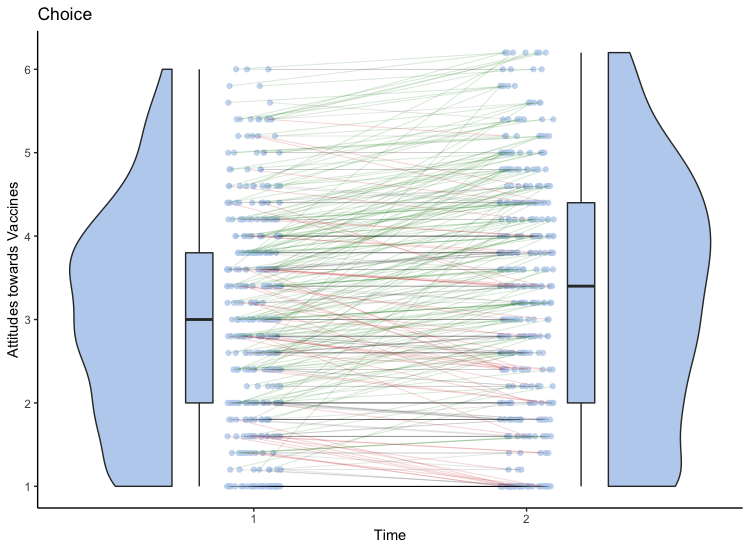
\includegraphics[width=0.75\linewidth]{../plots/ChoiceViolin} 

}

\caption{Example figure caption}\label{fig:examplefigurename}
\end{figure}

You can't see it, but in between this paragraph and the last we asked R to generate some random data and save it to a CSV file. Now we're going to import the data from the CSV file, as if it was independently created data - from an experiment or similar - and plot a graph.

\begin{figure}

{\centering 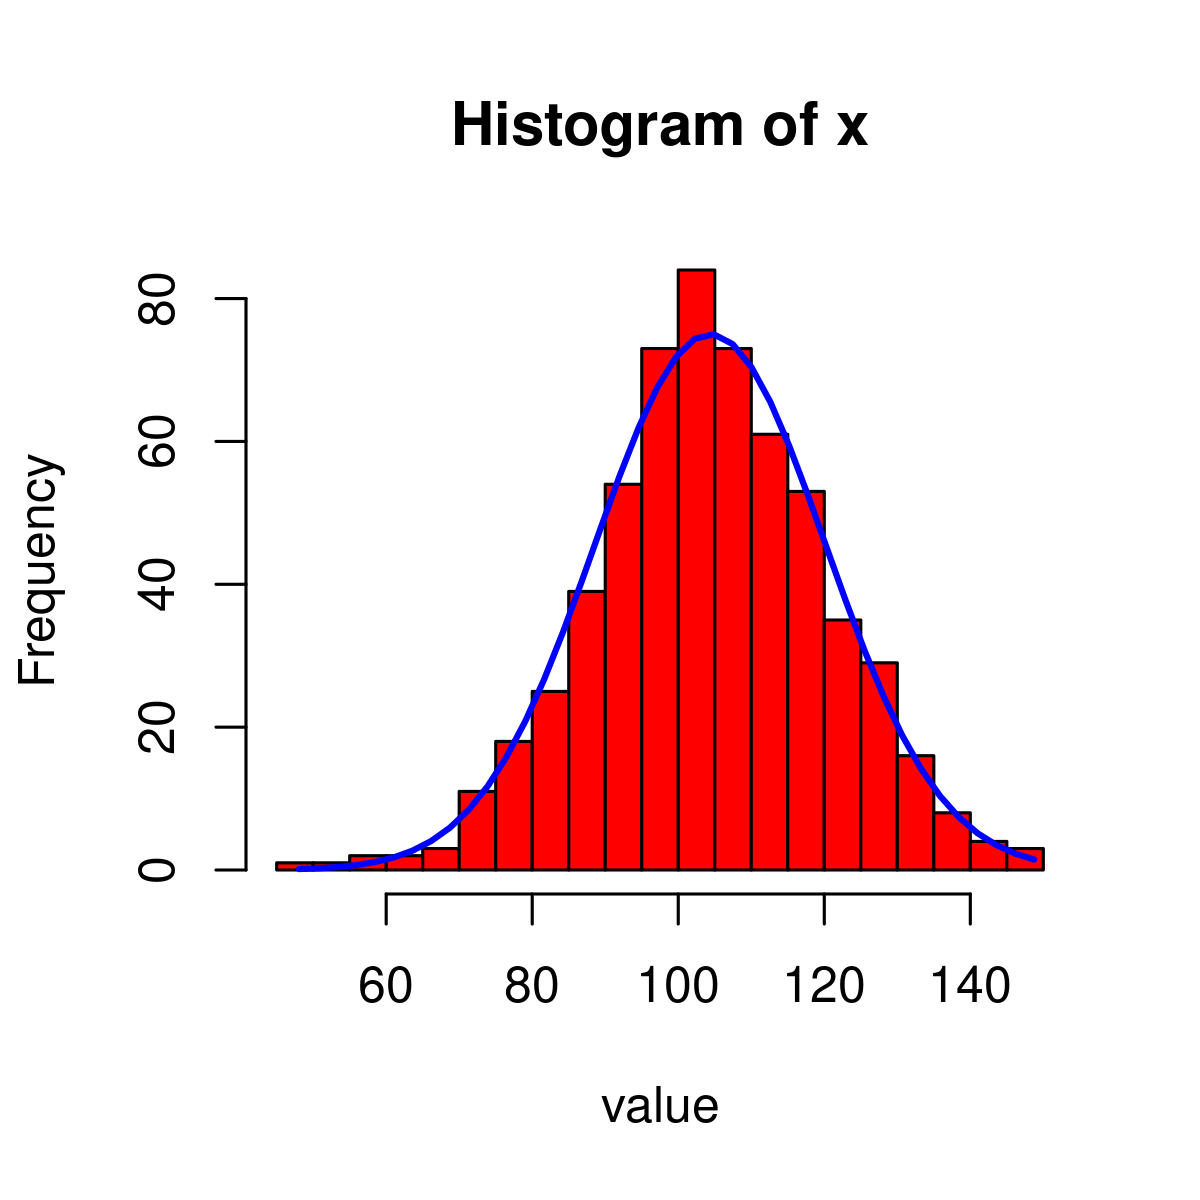
\includegraphics[width=0.75\linewidth]{clickbot_files/figure-latex/ourhistogram-1} 

}

\caption{Histogram of all data, grouped}\label{fig:ourhistogram}
\end{figure}

See Figure \ref{fig:ourhistogram}. Of course we could draw all sorts of things, but this is a proof-of-concept. Finally, let's run a t-test and integrate the results into the text.

mean = -1.75 and our credible intervals are from -0.57

We found there was a statistically significant difference between the two groups (t=-4.27 (592.62), p = 0.00). Note how the exact values in the previous sentence change every time we re-make the document (because the document also re-generates the underlying data).

Unanswered questions: Is this the best way to integrate values into text? Why is the df not an integer? What is the best way to define figure sizes so you get nice and/or consistent sizing across document formats?

\hypertarget{discussion}{%
\section{Discussion}\label{discussion}}

Make your document by opening .Rmd file in RStudio and clicking `knit'

Rmarkdown is good (Allaire et al., 2020). Need to change reference style? Change one line. Need to submit as PDF rather than .DOC? Just click `Word' as output rather than `PDF' (instructions here \url{https://rmarkdown.rstudio.com/articles_docx.html}). Need to change to two column style to make a nice pre-print? Again, simple - just change one line! In line 40 `class : ``man''\,' gives you manuscript style; ``jou'' gives you two column style.

To port to your own project just copy across these files:

\begin{itemize}
\tightlist
\item
  example\_manuscript.rmd
\item
  apa6.cls - style file which makes everything look APA format nice
\item
  references.bib - information on references in bibtex format
\item
  figs folder - where images integrated into the manuscript are kept
\end{itemize}

\hypertarget{main-conclusions}{%
\subsection{Main conclusions}\label{main-conclusions}}

Of course, there's more effort in installing and learning and correctly marking up your document in the first place, but it is worth it

\hypertarget{references}{%
\section*{References}\label{references}}
\addcontentsline{toc}{section}{References}

\hypertarget{refs}{}
\begin{CSLReferences}{1}{0}
\leavevmode\vadjust pre{\hypertarget{ref-rmarkdowncite}{}}%
Allaire, J., Xie, Y., McPherson, J., Luraschi, J., Ushey, K., Atkins, A., \ldots{} Iannone, R. (2020). \emph{Rmarkdown: Dynamic documents for r}. Retrieved from \url{https://github.com/rstudio/rmarkdown}

\leavevmode\vadjust pre{\hypertarget{ref-aust2020}{}}%
Aust, F., \& Barth, M. (2020). \emph{{papaja}: {Create} {APA} manuscripts with {R Markdown}}. Retrieved from \url{https://github.com/crsh/papaja}

\leavevmode\vadjust pre{\hypertarget{ref-heitz2014speed}{}}%
Heitz, R. P. (2014). The speed-accuracy tradeoff: History, physiology, methodology, and behavior. \emph{Frontiers in Neuroscience}, \emph{8}, 150.

\leavevmode\vadjust pre{\hypertarget{ref-mcelreath2018statistical}{}}%
McElreath, R. (2018). \emph{Statistical rethinking: A bayesian course with examples in r and stan}. Chapman; Hall/CRC.

\leavevmode\vadjust pre{\hypertarget{ref-stafford2020}{}}%
Stafford, T., Pirrone, A., Croucher, M., \& Krystalli, A. (2020). Quantifying the benefits of using decision models with response time and accuracy data. \emph{Behavior Research Methods}, \emph{52}, 2142-\/-2155.

\leavevmode\vadjust pre{\hypertarget{ref-wickelgren1977speed}{}}%
Wickelgren, W. A. (1977). Speed-accuracy tradeoff and information processing dynamics. \emph{Acta Psychologica}, \emph{41}(1), 67--85.

\end{CSLReferences}


\end{document}
